\documentclass{classes/mybeamer}

\DeclareMathOperator{\rank}{rank}
\DeclareMathOperator{\NS}{NS}
\DeclareMathOperator{\Tr}{Tr}
\DeclareMathOperator{\chara}{char}
\DeclareMathOperator{\Spec}{Spec}
\DeclareMathOperator{\ch}{ch}
\newcommand{\Neron}{N\'eron}

\title{2次Frey曲線に付随する楕円曲面のMordell-Weil群について}
\subtitle{On the Mordell-Weil groups of elliptic surfaces associated with Frey curves of degree two}
\author{八木 颯仁}
\institute{慶應義塾大学 栗原研究室 修士2年}
\date{February 7, 2025}

\begin{document}

\begin{frame}
    \titlepage
\end{frame}

\begin{frame}{発表の概要と動機}
    \begin{dfn*}
        Fermat 方程式
        \begin{equation*}
            x^n + y^n = z^n, \quad xyz \neq 0, \quad n \geq 2
        \end{equation*}
        の整数解$(x, y, z)=(a,b,c)$に対し、
        \begin{equation*}
            y^2 = x (x-a^n) (x+b^n)
        \end{equation*}
        は楕円曲線を与える。これを\color{blue}\textbf{Frey 曲線}\color{black}と呼ぶ。
    \end{dfn*}
    本研究では $n=2$ の場合の Frey 曲線の族について、それらをまとめて一つの\textbf{楕円曲面}と結び付けて扱うことで、 Mordell-Weil 群の構造についていくつかの結果を得た。
    \begin{itemize}
        \item ランク $0$ の2次 Frey 曲線はたくさん見つかるが、ランクが $1$ の例もいくつか見つかっている。ランクが正の 2次 Frey 曲線は無限個存在するのか?
        \item ランクが正の族を具体的にパラメトライズされた形で構成できないか?
    \end{itemize}
    \vspace{1em}
    \tableofcontents
\end{frame}

\section{Introduction}
\begin{frame}{楕円曲線とは}
    体$K$ (標数 $\neq2$ とする)上の\color{blue}\textbf{楕円曲線}\color{black}$E$とは次のような形の方程式で表される曲線である。
    \begin{equation*}
        E: y^{2} = x^{3} + Ax^2 + Bx + C \quad (A,B,C \in K)
    \end{equation*}
    ただし判別式 $\Delta = -4A^3C + A^2B^2 + 18ABC - 4B^3 - 27C^2$ は $0$ でないとする。

    \vspace{1cm}

    楕円曲線上の $K$-有理点全体は群をなし、$E(K)$ と書いて\color{blue}\textbf{Mordell-Weil 群}\color{black}と呼ぶ。
    Mordell-Weil の定理によると、$K$ に関する仮定の下で $E(K)$ は有限生成アーベル群である。
    したがって
    \begin{equation*}
        E(K) \cong \mathbb{Z}^{\oplus r} \oplus E(K)_{\mathrm{tors}}
    \end{equation*}
    と書ける。ここで $r$ は\color{blue}\textbf{ランク}\color{black}、$E(K)_{\mathrm{tors}}$ は\color{blue}\textbf{捩れ部分群}\color{black} (torsion subgroup) と呼ばれる。
\end{frame}

% \begin{frame}
%     \begin{figure}[htbp]
%         \centering
%         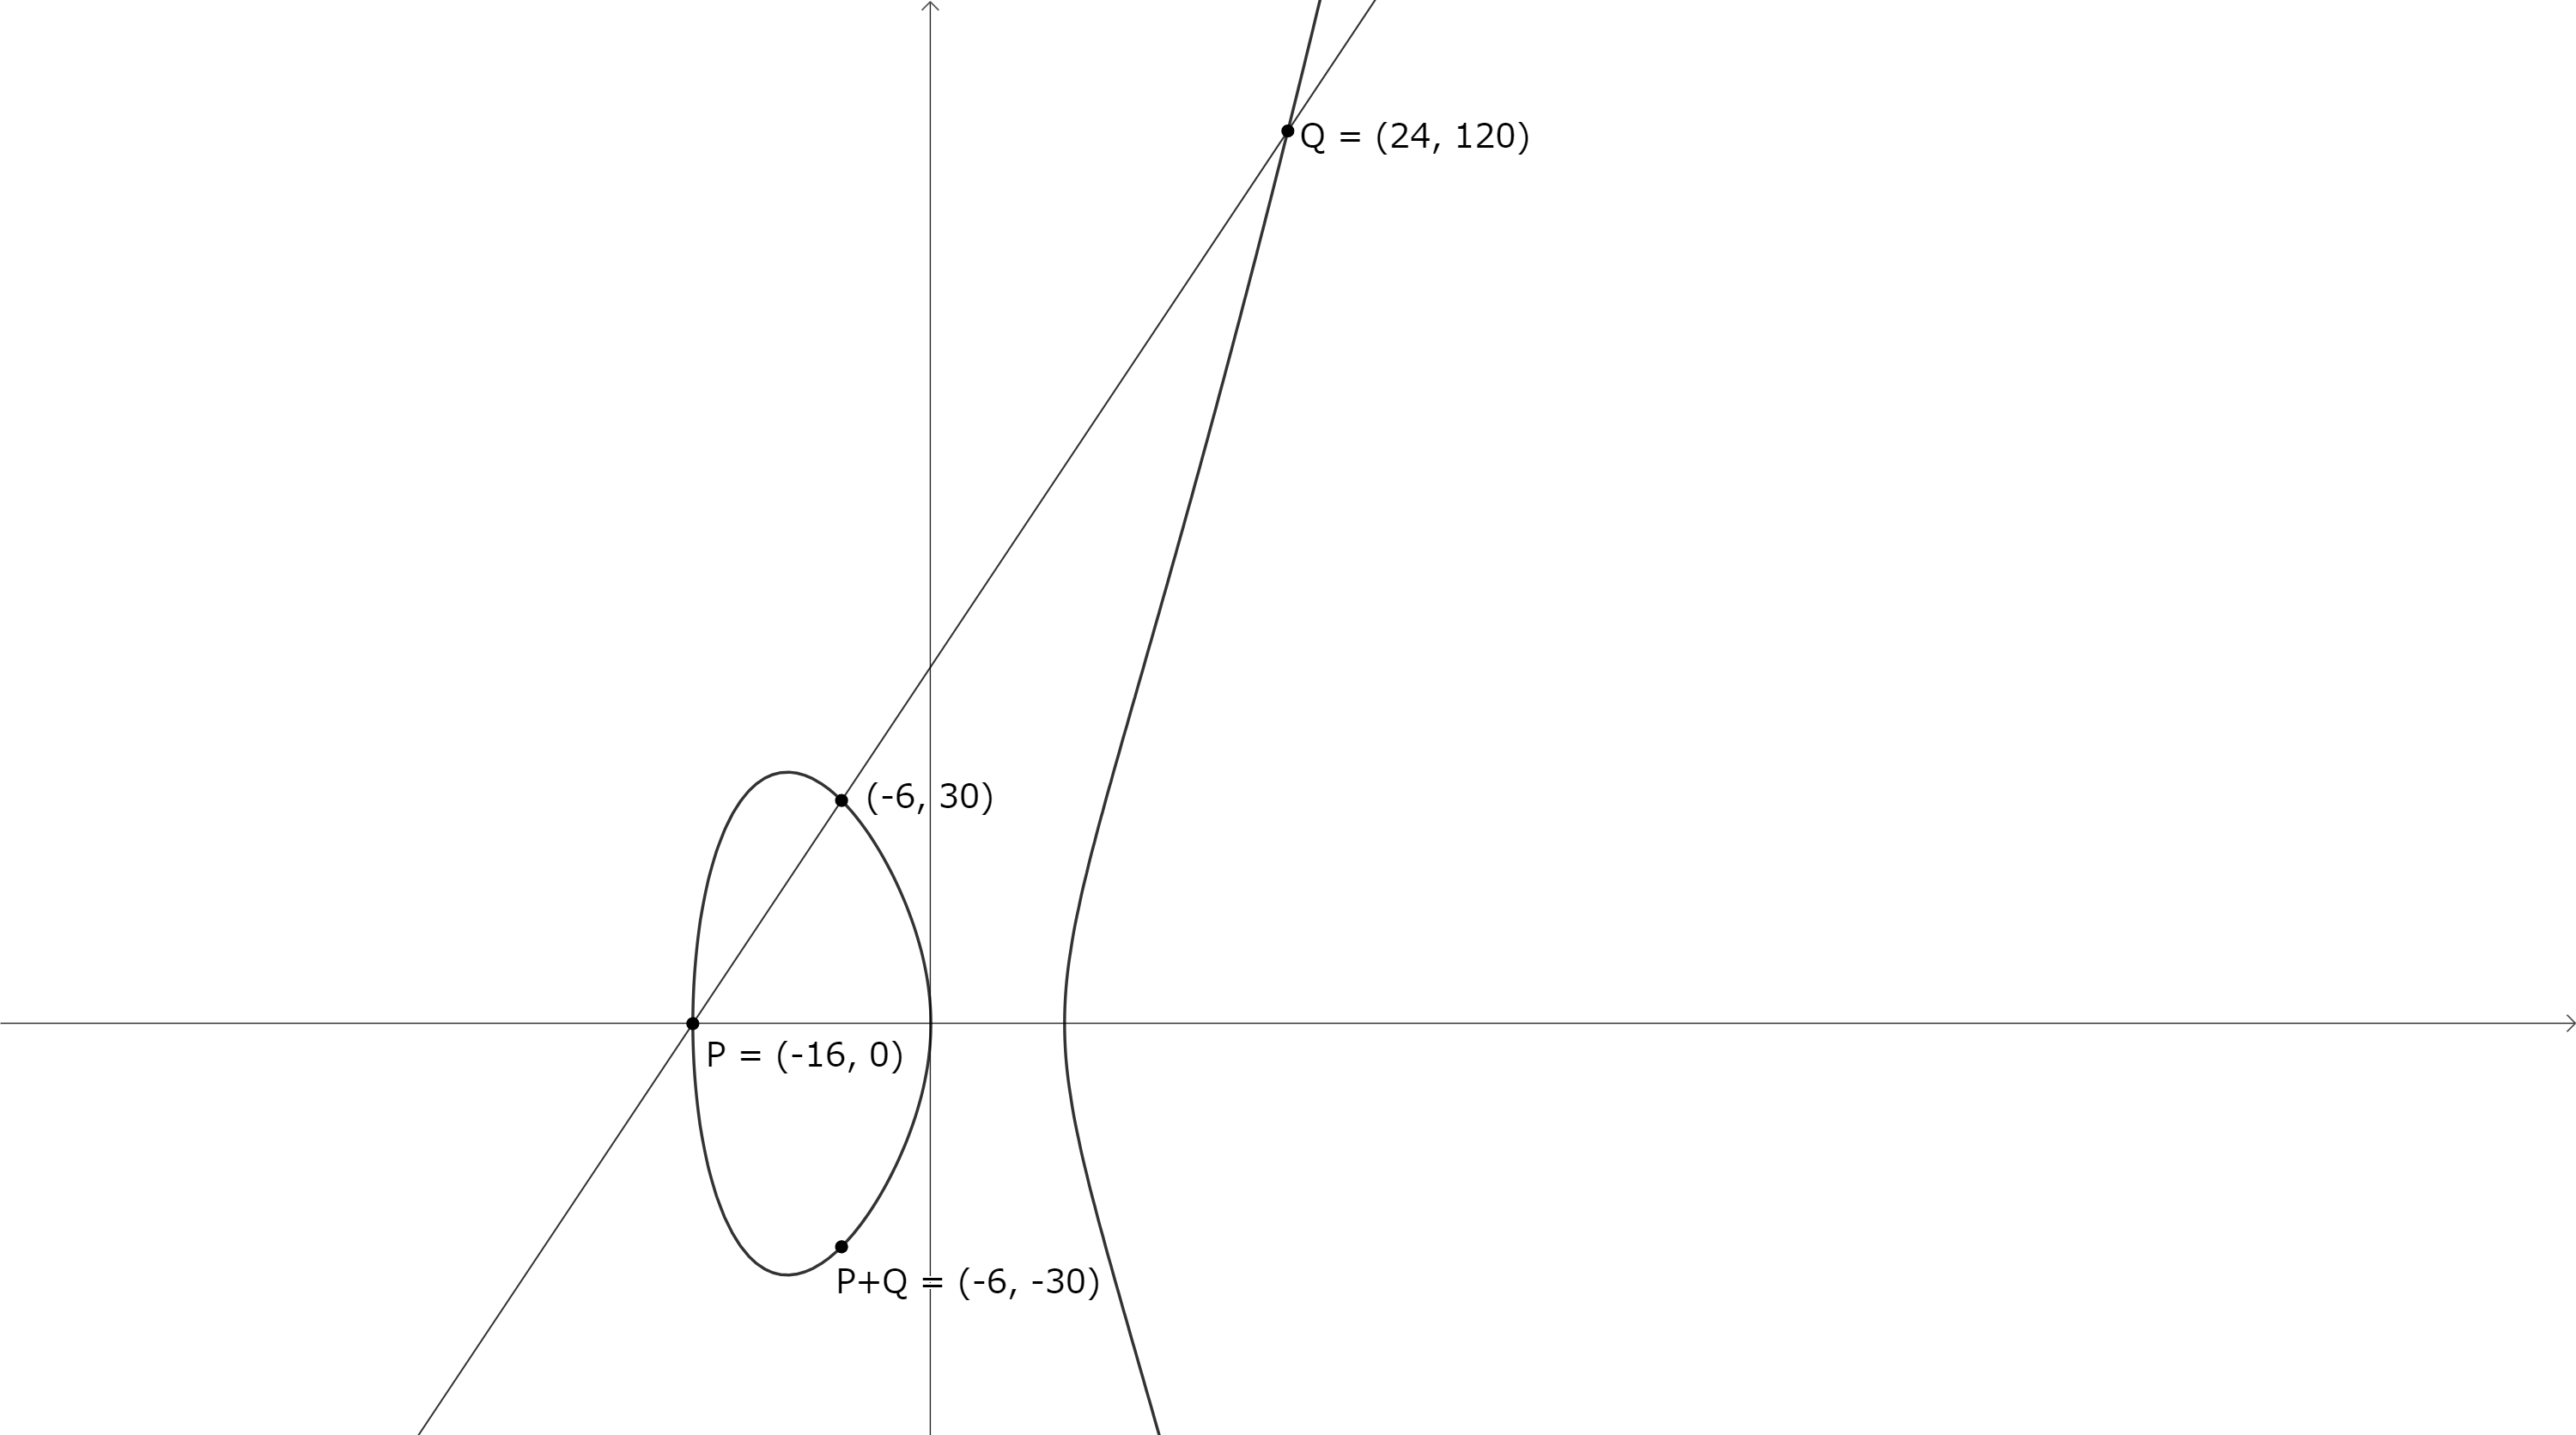
\includegraphics[keepaspectratio, height=8.5cm]{figures/3-4-5.png}
%         \vspace{-1.5cm}
%         \caption{
%             \rightline{
%                 $E: y^2 = x(x-3^2)(x+4^2)$
%             }
%         }
%     \end{figure}
% \end{frame}


\begin{frame}{2次 Frey 曲線}
    本研究では Frey 曲線の$2$次の場合を扱う。
    \begin{dfn*}
        $(a,b,c)$を以下を満たす正整数の$3$つ組とする。
        \begin{equation*}
            \label{eq:pythagorean_triple}
            a^2+b^2=c^2.
        \end{equation*}
        そのような $(a,b,c)$ に対し、次の方程式で与えられる楕円曲線$E/\mathbb{Q}$を考える。
        \begin{equation*}
            \label{eq:2frey}
            E: y^2 = x (x-a^2) (x+b^2)
        \end{equation*}
    \end{dfn*}
    $(a,b,c)$ が互いに素でない場合は適当な変数変換によって原始ピタゴラス数の場合に帰着できる。
    原始ピタゴラス数 $(a,b,c)$ は$2$つの互いに素な正整数 $m > n$ によって
    \begin{equation*}
        (a,b,c) = (2mn, m^{2} - n^{2}, m^{2} + n^{2})
    \end{equation*}
    とパラメトライズされる。
    これを上の式に代入すると $y^{2} = x(x - 4m^2n^2)(x + (m^{2} - n^2)^{2})$ と書け、
    $x,y$ を $n^2x, n^3y$ で置き換えて $s = m/n$ とおくと
    \begin{eg*}
        \begin{equation*}
            \label{eq:E_{1,s}}
            E_{1,s}: y^{2} = x(x - 4s^{2})(x + (s^{2} - 1)^{2})
        \end{equation*}
    \end{eg*}
    という方程式を得る。    
\end{frame}

\begin{frame}
    \begin{eg*}
        \begin{equation*}
            E_{1,s}: y^{2} = x(x - 4s^{2})(x + (s^{2} - 1)^{2})
        \end{equation*}
    \end{eg*}
    本研究では、$s$ に値を代入した個々の楕円曲線について考える代わりに、 $E_{1,s}$ を\textbf{関数体} $\overline{\mathbb{Q}}(s)$ \textbf{上の楕円曲線}として考える。
    さらに$E_{1,s}$ に対して
    \begin{equation*}
        \mathcal{E}_{1} = \left\{ ([X,Y,Z],s_0) \in \mathbb{P}^{2} \times \mathbb{P}^{1} \mid Y^{2}Z = X(X - 4s_{0}^{2}Z)(X + (s_{0}^{2} - 1)^{2}Z) \right\}
    \end{equation*}
    という $\mathbb{P}^{2} \times \mathbb{P}^{1}$ の$2$次元部分多様体を考えることで、$E_{1,s}$ に対して\textbf{楕円曲面} $\pi: \mathcal{E}_{1}\to \mathbb{P}^{1}$ \textbf{を対応させる}ことができる。
    $E_{1,s}$ を $\mathcal{E}_{1} \to \mathbb{P}^{1}$ の generic fiber と呼び、 $\mathcal{E}_{1,s_0}:=\pi^{-1}(s_0)$ を special fiber と呼ぶ。
    有限個を除きすべての special fibers は非特異、すなわち楕円曲線である。
    \begin{figure}[htbp]
        \centering
        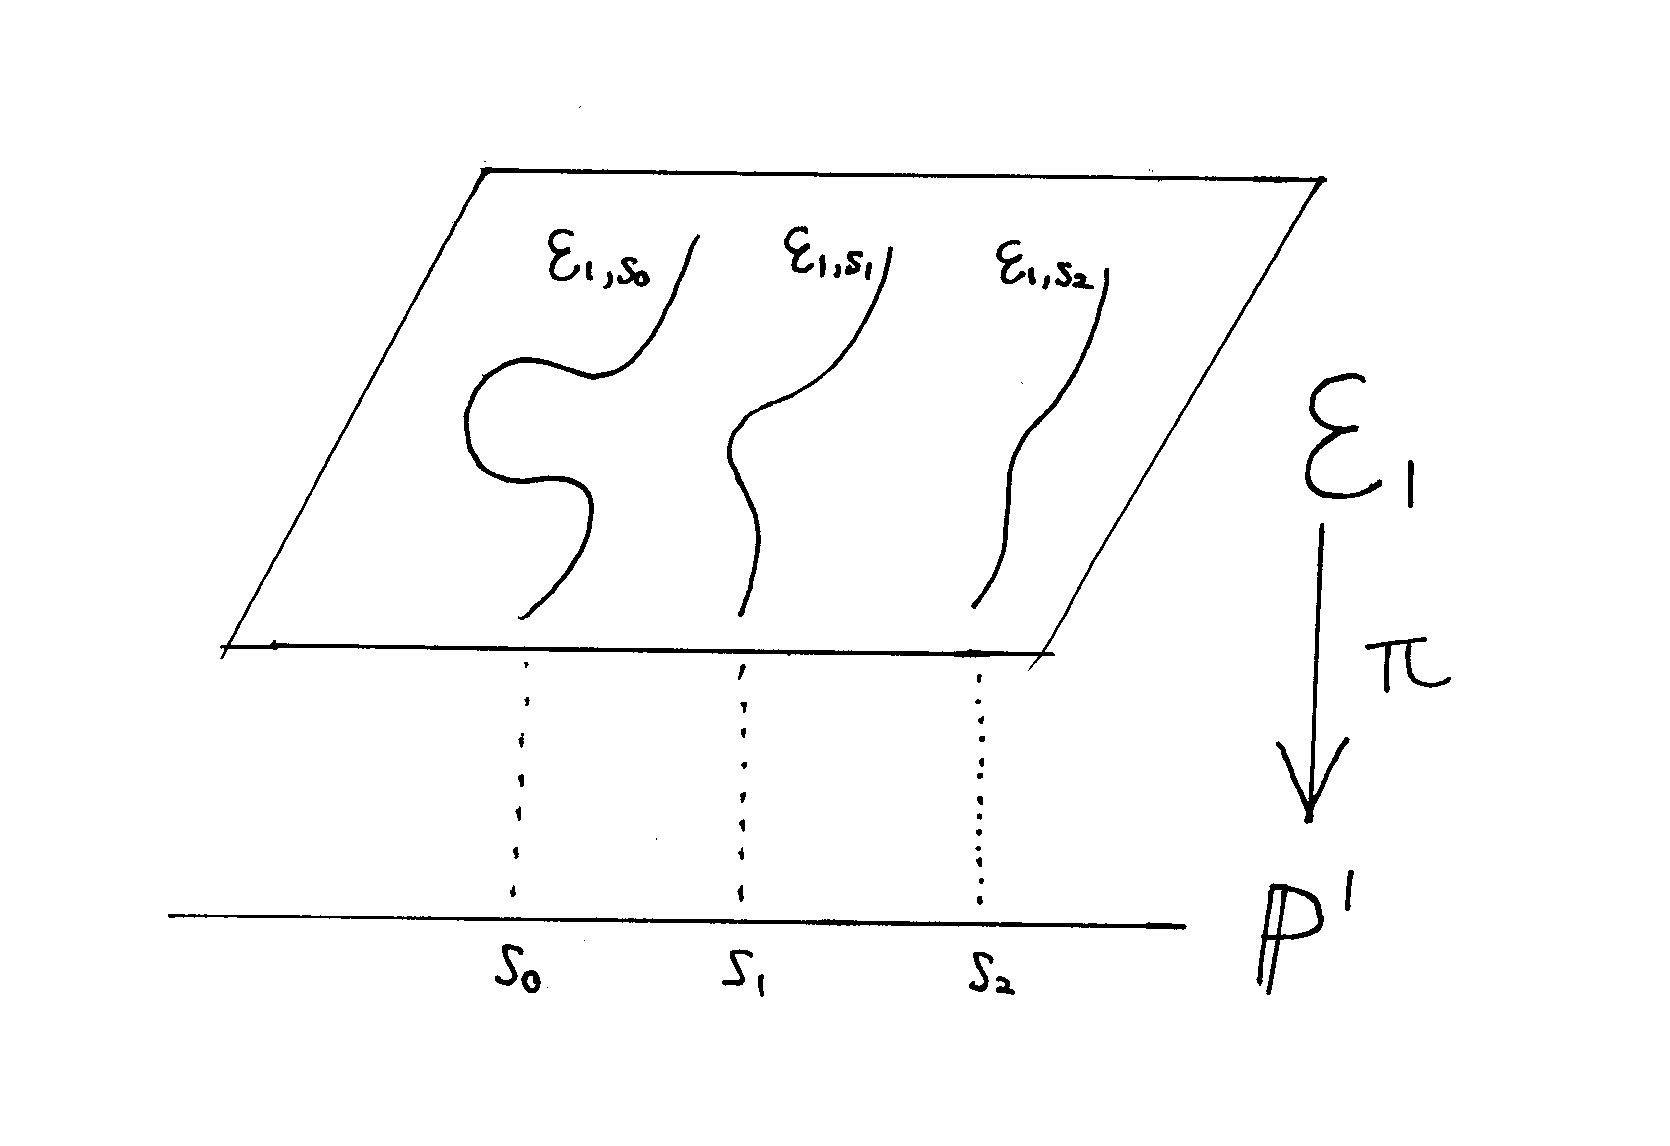
\includegraphics[keepaspectratio, height=4.5cm]{figures/elliptic_surface.jpg}
    \end{figure}
\end{frame}

\section{主定理}
\begin{frame}{主定理}
    \begin{proposition}[Y.]
        \begin{equation*}
            E_{1,s}(\overline{\mathbb{Q}}(s)) \cong \mathbb{Z} / 4 \mathbb{Z} \oplus \mathbb{Z} / 4 \mathbb{Z},
        \end{equation*}
    \end{proposition}
    \vspace{1em}
    
    $E_{1,s}$ に $s = \frac{2t}{t^{2} - 3}$ を代入して
    \begin{equation*}
        E_{2,t}: y^{2} = x \left(x - 4 \left(\frac{2t}{t^{2} - 3} \right)^{2} \right) \left(x + \left(\left(\frac{2t}{t^{2} - 3} \right)^{2} - 1 \right)^{2} \right),
    \end{equation*}
    という $E_{1,s}$ の部分族を考える。
    \begin{thm}[Y.]
        \begin{equation*}
            E_{2,t}(\overline{\mathbb{Q}}(t)) \cong \mathbb{Z} \oplus \mathbb{Z} / 4 \mathbb{Z} \oplus \mathbb{Z} / 4 \mathbb{Z},
        \end{equation*}
        % The torsion subgroup is generated by $T_1$ and $T_2$ in Theorem~\ref{thm:E_{1,s}} with $s = \frac{2t}{t^{2} - 3}$.
    \end{thm}
    ここでランクがちょうど$1$であることを示したということが重要である。
\end{frame}

\begin{frame}{Specialization Theorem}
    関数体上の Mordell-Weil 群と special fiber の Mordell-Weil 群の間には以下の関係がある。
    \begin{thm}[Specialization Theorem, \cite{ref:advancedaec}]
        \label{thm:specialization}
        \begin{itemize}
            \item $\pi:\mathcal{E} \to \mathbb{P}^1$ を $\mathbb{Q}$ 上の non-split な楕円曲面
            \item $E$ を対応する $\mathbb{Q}(\mathbb{P}^1)$ 上の楕円曲線
            \item $\mathcal{E}_s:=\pi^{-1}(s)$ を $s$ での special fiber
        \end{itemize}
        とする。
        このとき有限個を除くすべての $s \in \mathbb{P}^1(\overline{\mathbb{Q}})$に対して specialization homomorphism
        \begin{equation*}
            E(\overline{\mathbb{Q}}(\mathbb{P}^1)) \hookrightarrow \mathcal{E}_{s}(\overline{\mathbb{Q}})
        \end{equation*}
        が定義できて、これは\textbf{単射}である。
    \end{thm}
    特に有限個の点を除き generic fiber のランクより special fiber のランクが小さくなることはない。
    したがって関数体上でランクの高い楕円曲線を見つけると、 $s$ に値を代入することで$\overline{\mathbb{Q}}$上ランクの高い楕円曲線を無限個見つけることができる。
\end{frame}

\section{証明の概要}
\begin{frame}{証明の概要}
    \begin{itemize}
        \item 捩れ部分群についての証明はランクに比べて簡単なのでここでは省略する。
        \item $E_{2,t}$上の点
            \begin{equation*}
                \left(s^{2} - 1, \sqrt{-1} s(s^{2} - 1) \frac{t^{2} + 3}{t^{2} - 3} \right) \in E_{2,t}(\overline{\mathbb{Q}}(t)) \setminus E_{2,t}(\overline{\mathbb{Q}}(t))_{\text{tors}}.
            \end{equation*}
            は無限位数の点であることから $E_{2,t}(\overline{\mathbb{Q}}(t))$ のランクは$1$以上であることが分かる。
        \item 重要なのは $E_{1,s}(\overline{\mathbb{Q}}(s))$ のランクが $0$ 以下、 $ E_{2,t}(\overline{\mathbb{Q}}(t))$ のランクが$1$以下であることを示すことである。
    \end{itemize}

    \vspace{1cm}

    証明は大きく2つのステップに分けられる。
    \begin{enumerate}
        \item Mordell-Weil 群のランクと Picard 数(後述)の関係を調べる。
        \item Picard 数を上から不等式で評価する。
    \end{enumerate}
\end{frame}

\begin{frame}{Shioda-Tate formula}
    \begin{thm}[Shioda-Tate formula, \cite{ref:shioda1990}]
        \label{thm:shioda}
        \begin{itemize}
            \item $\mathcal{E} \to \mathbb{P}^1$ を代数閉体 $k$ 上で定義された楕円曲面
            \item $R \subset \mathbb{P}^1$ をその上の special fiber が特異となる点全体の集合
            \item 各 $v \in R$ に対し、 $m_{v}$ を $v$ の上の special fiber の既約成分の数
            \item $\rho(\mathcal{E})$ を $\mathcal{E}$ の \Neron-Severi 群のランク( Picard 数と呼ばれる)
        \end{itemize}
        とする。
        このとき
        \begin{equation*}
            \rho (\mathcal{E}) = 2 + \sum_{v \in R} (m_{v} - 1) + \rank(E(k(\mathbb{P}^1)))
        \end{equation*}
        が成り立つ。
    \end{thm}
    定理中に現れる $R$ や $m_v$ は Tate's algorithm によって計算できる。
\end{frame}

\begin{frame}{Picard 数の評価}
    \begin{proposition}[\cite{ref:naskreckiphd}]
        \begin{itemize}
            \item $k$ と $\mathcal{E} \to \mathbb{P}^1$ と $R$ は先ほどの定理 (Shioda-Tate formula) と同じもの
            \item 各 $v \in R$ に対し、$e(\mathcal{E}_v)$ を special fiber $\mathcal{E}_v$ の Euler 数
        \end{itemize}
        とする。
        このとき
        \begin{equation*}
            \rho(\mathcal{E}) \leq \frac{5}{6} \sum_{v \in R} e(\mathcal{E}_v)
        \end{equation*}
        が成り立つ。
    \end{proposition}
    $e(\mathcal{E}_v)$ も Tate's algorithm によって計算できる。
\end{frame}

\begin{frame}{$E_{1,s}(\overline{\mathbb{Q}}(s))$ のランク}
    実際 Tate's algorithm により各値は以下のように計算できる。
    \begin{table}[htbp]
        \centering
        \caption{$E_{1,s}$ の特異ファイバー}
        \begin{tabular}{|c|c|c|c|}
            \hline
            Place             & Type  & $m_v$ & $e$ \\
            \hline
            $s=0$             & $I_4$ & 4     & 4   \\
            $s=\pm 1$         & $I_4$ & 4     & 4   \\
            $s=\pm \sqrt{-1}$ & $I_4$ & 4     & 4   \\
            $s=\infty$        & $I_4$ & 4     & 4   \\
            \hline
        \end{tabular}
    \end{table}
    したがって $\rho(E_{1,s}) \leq 20$ であり、 $\rank(E_{1,s}(\overline{\mathbb{Q}}(s))) \leq 0$ であることが分かる。
\end{frame}

\begin{frame}{$E_{2,t}(\overline{\mathbb{Q}}(t))$ のランク}
    ところが、同じ計算を $E_{2,t}$ に対して行っても、ランクが2以下であることしか分からない。
    Picard 数の評価がゆるい。別の方法でより良い評価を得る必要がある。その準備として次の定理が必要である。
    \begin{thm}[Y.]
        \begin{equation*}
            E_{0,u}: y^{2} = x(x - 4u)(x + (u - 1)^{2})
        \end{equation*}
        という $\overline{\mathbb{Q}}(u)$ 上の楕円曲線を新たに用意する。
        $E^{(w)}$ で $E$ の $w$ での quadratic twist を表す。
        このとき
        \begin{equation*}
            \begin{split}
                \rank E_{2,t}(\overline{\mathbb{Q}}(t)) & = \rank E_{1,s}(\overline{\mathbb{Q}}(s))                \\
                                                        & + \rank E_{0,u}^{(1 + 3u)}(\overline{\mathbb{Q}}(u))     \\
                                                        & + \rank E_{0,u}^{(u(1 + 3u))}(\overline{\mathbb{Q}}(u)).
            \end{split}
        \end{equation*}
    \end{thm}
    既に $E_{1,s}$ のランクが $0$ であることが分かっている。
    また $E_{0,u}^{(u(1 + 3u))}$ のランクが $1$ であることも同じ方法で分かる。
    残るは $E_{0,u}^{(1 + 3u)}$ のランクを計算することである。
    $E_{0,u}^{(1 + 3u)}$ は $E_{2,t}$ より係数の次数が低く、また対応する楕円曲面が\textbf{K3曲面}と呼ばれるよく研究された対象になることから、この後の計算が実行可能になる。
\end{frame}

\begin{frame}
    \begin{itemize}
        \item $p$を素数、 $q$ を $p$ の冪とする。
        \item $S:=\mathcal{E}_{0}^{(1 + 3u)}\to \mathbb{P}^{1}$ に対して $\tilde{S} = S_{\overline{\mathbb{F}_q}} \to \mathbb{P}^1$ という reduction を考えることができる。
        \item $l$ を $p$ と異なる素数として $l$-進 \'etale コホモロジーを $H^{i}_{\text{\'et}}(\tilde{S}, \mathbb{Q}_l)$ と書く。
        \item $H^{i}_{\text{\'et}}(\tilde{S}, \mathbb{Q}_l)$に作用する Frobenius 自己同型を $\varphi^{(i)}$ と書く。
    \end{itemize}
    このとき $\tilde{S}$ に関するいくつかの仮定の下で以下の定理が成り立つ。
    \begin{thm}[\cite{ref:vanluijk2007}]
        \label{cor:ns_upper_bound}
        $S$ や $\tilde{S}$の \Neron-Severi 群のランクは、$\varphi^{(2)}$ の固有値 $\lambda$ で $\lambda/q$ が$1$のべき根であるようなものの重複度を込めた個数以下である。
    \end{thm}
    $\varphi^{(2)}$ の固有多項式を求めるには、今の場合 $m=1,2,3$ に対して $\Tr((\varphi^{(2)})^m)$ を計算すればよい。
    \begin{thm}[Lefschetz の不動点定理]
        \begin{equation*}
            \# \tilde{S}(\mathbb{F}_{q^{m}}) = \sum_{i = 0}^{n} ( - 1)^{i} \Tr((\varphi^{(i)})^{m}).
        \end{equation*}
    \end{thm}
\end{frame}

\begin{frame}
    $q=5$ として実際に計算すると
    \begin{table}[ht]
        \centering
        \caption{Singular fibers of $E_{0,u}^{(1 + 3u)}$}
        \begin{tabular}{|c|c|c|c|}
            \hline
            Place            & Type    & $m_v$ & $e$ \\
            \hline
            $u=0$            & $I_2$   & 2     & 2   \\
            $u=\pm 1$        & $I_4$   & 4     & 4   \\
            $u=-\frac{1}{3}$ & $I_0^*$ & 5     & 6   \\
            $u=\infty$       & $I_2^*$ & 7     & 8   \\
            \hline
        \end{tabular}
        \label{tab:E_{0,u}^{(1 + 3u)}}
    \end{table}

    \begin{table}[ht]
        \centering
        \caption{$\# \tilde{S}(\mathbb{F}_{5^{m}})$}
        \begin{tabular}{|c|c|c|c|}
            \hline
            $m$                              & 1   & 2    & 3     \\
            \hline
            $\# \tilde{S}(\mathbb{F}_{5^m})$ & 120 & 1080 & 18264 \\
            \hline
            % $t_m$                            & -1  & -21  & 263   \\
            % \hline
        \end{tabular}
        \label{tab:tm}
    \end{table}
    これらの計算により固有多項式は
    \begin{equation*}
        \chara(\varphi^{(2)}) = (x - 5)^{19}(x^{3} + x^{2} + 11 x - 77)
    \end{equation*}
    と計算でき、 $\rho(\mathcal{E}_{0,u}^{(1 + 3u)}) \leq 19$ と分かる。
    Shioda-Tate formula により $\rank E_{0,u}^{(1 + 3u)}(\overline{\mathbb{Q}}(u)) \leq 0$ が従い、主定理のランク部分である $\rank E_{2,t}(\overline{\mathbb{Q}}(t)) = 1$ が得られる。
\end{frame}

\begin{frame}
    \begin{table}[H]
        \centering
        \caption{Number of points on each singular fiber over a finite field}
        \begin{tabular}{|c|c|c|c|}
            \hline
            Type             & Configuration                                                                      & $m_v$ & $\mathcal{E}_v(\mathbb{F}_{q^{m}})$ \\
            \hline
            $\mathrm{I}_n$   & \raisebox{-0.5 \height}{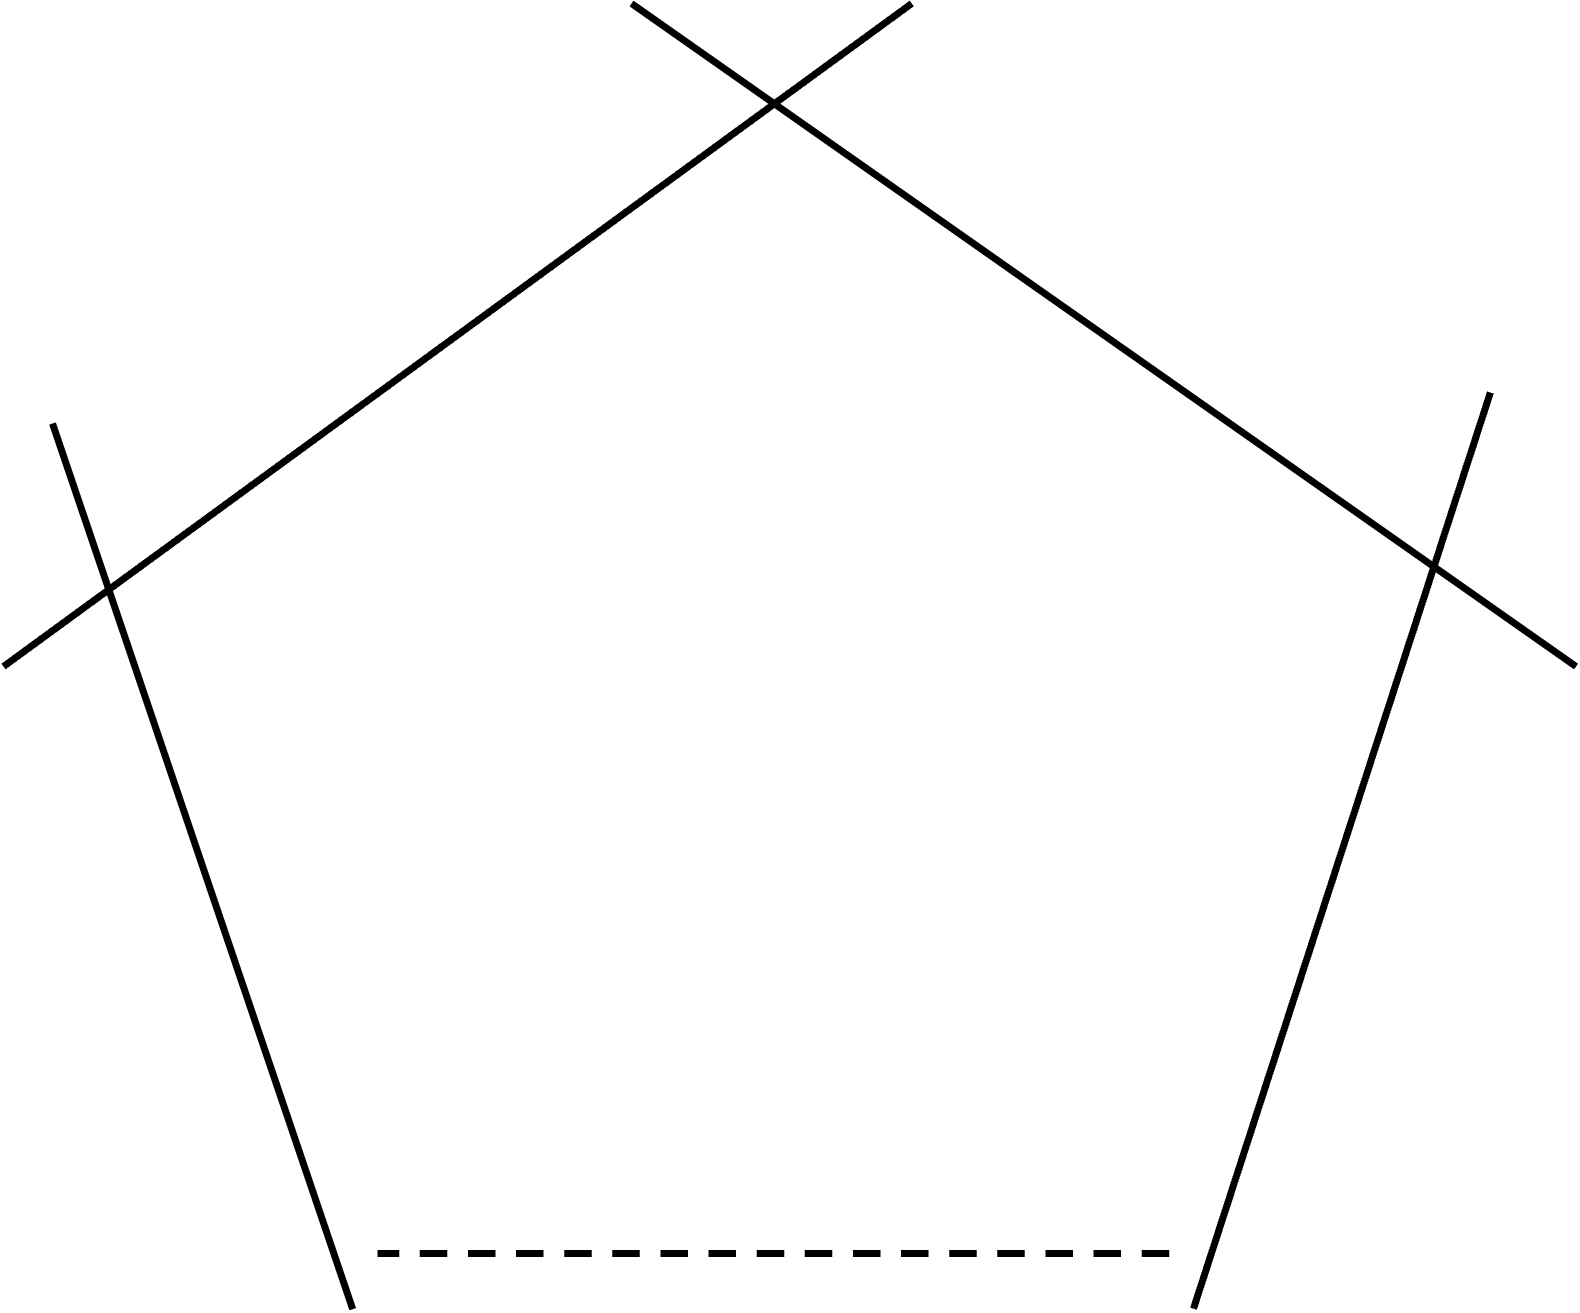
\includegraphics[width=4cm, height=3cm]{figures/I_n.png}}  & $n$   & $nq^m$                              \\
            $\mathrm{I}_n^*$ & \raisebox{-0.5 \height}{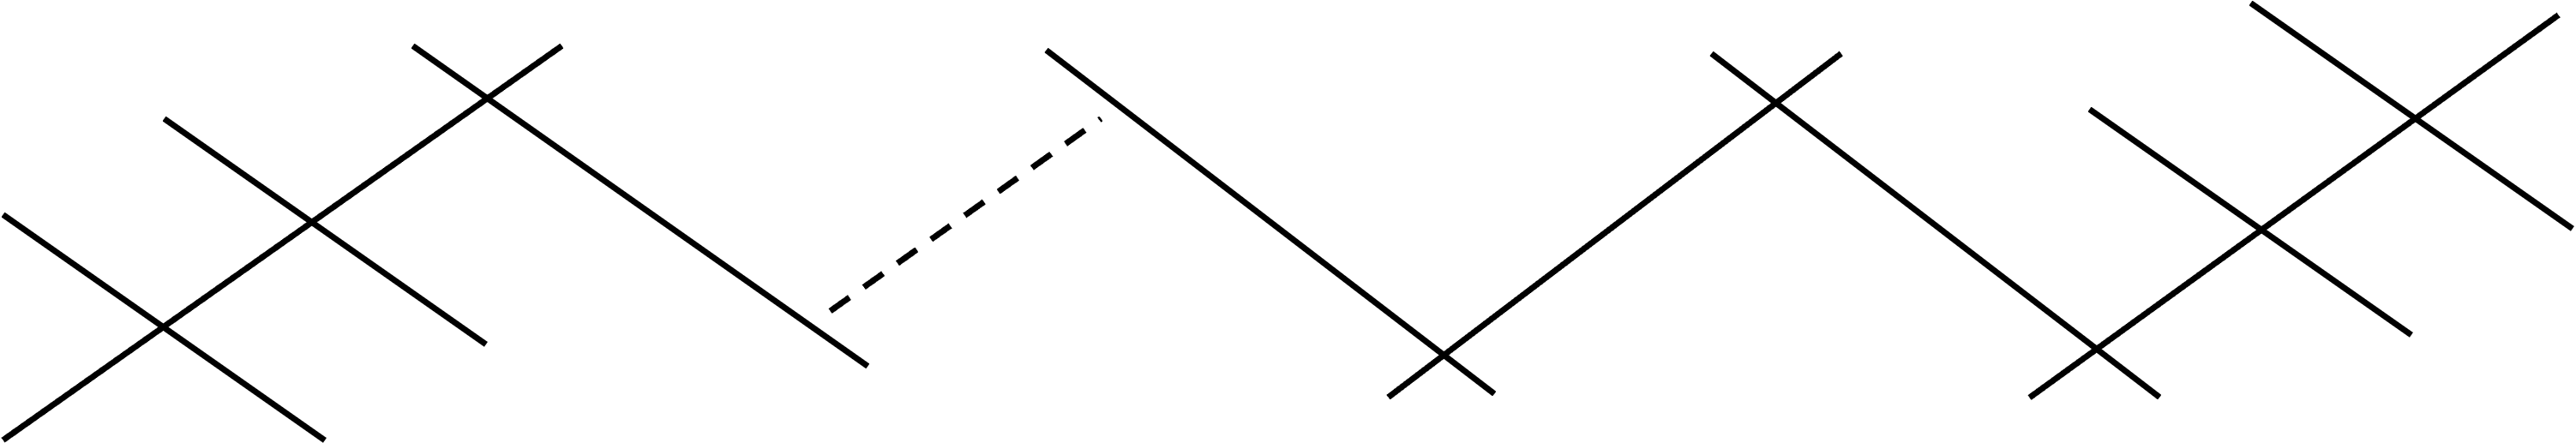
\includegraphics[width=4cm, height=2cm]{figures/I_nx.png}} & $n+5$ & $(n+5) q^m+1$                       \\
            \hline
        \end{tabular}
        \label{tab:reductionpoints}
    \end{table}
\end{frame}

\begin{frame}{参考文献}
    \scriptsize
    \beamertemplatetextbibitems
    \bibliographystyle{jplain}
    \bibliography{references}
\end{frame}
\end{document}
